\chapter{Results and Analysis} \label{ch:results-analysis}

We demonstrate the output of the Frangi filter on our samples after running a multiscale technique with $N=20$ scales with a stricter anisotropy parameter $\beta = 0.35$ and standard structureness parameter $\gamma=0.5$,
with scales spaced logarithmically from $\sigma_1 = 2^{-1}$ to $\sigma_N = 2^{3.5}$, performing glare and cut removal in preprocessing, and using a discrete gaussian kernel and dilation border of 20.
Our goal in this section is to provide a close up look at the Frangi filter on two samples, and then provide some measures of the Frangi output's correspondence with the ``ground truth'' network tracings across all 201 images, without explicitly performing segmentation. However, for visual demonstration, we will employ both simple thresholding techniques (arbitrary fixed and nonzero-percentile) described in \cref{ch:multifrangi}. In \cref{ch:segmentation} we will develop and analyze more sophisticated Frangi-based segmentation techniques and compare their performance to these rudimentary thresholding techniques across the entire dataset.

\section{Sample visual output}
In \cref{fig:output-montage-example1} and \cref{fig:output-montage-example2} we take a look at the Frangi output (\Vmax) for two particularly well-behaved samples. In the top-left, the preprocessed placenta is shown. In the top-right, the maximum of the Frangi output over $N$ scales. The bottom left and right images are two rudimentary thresholds of $\Vmax$.

\begin{figure} \centering
  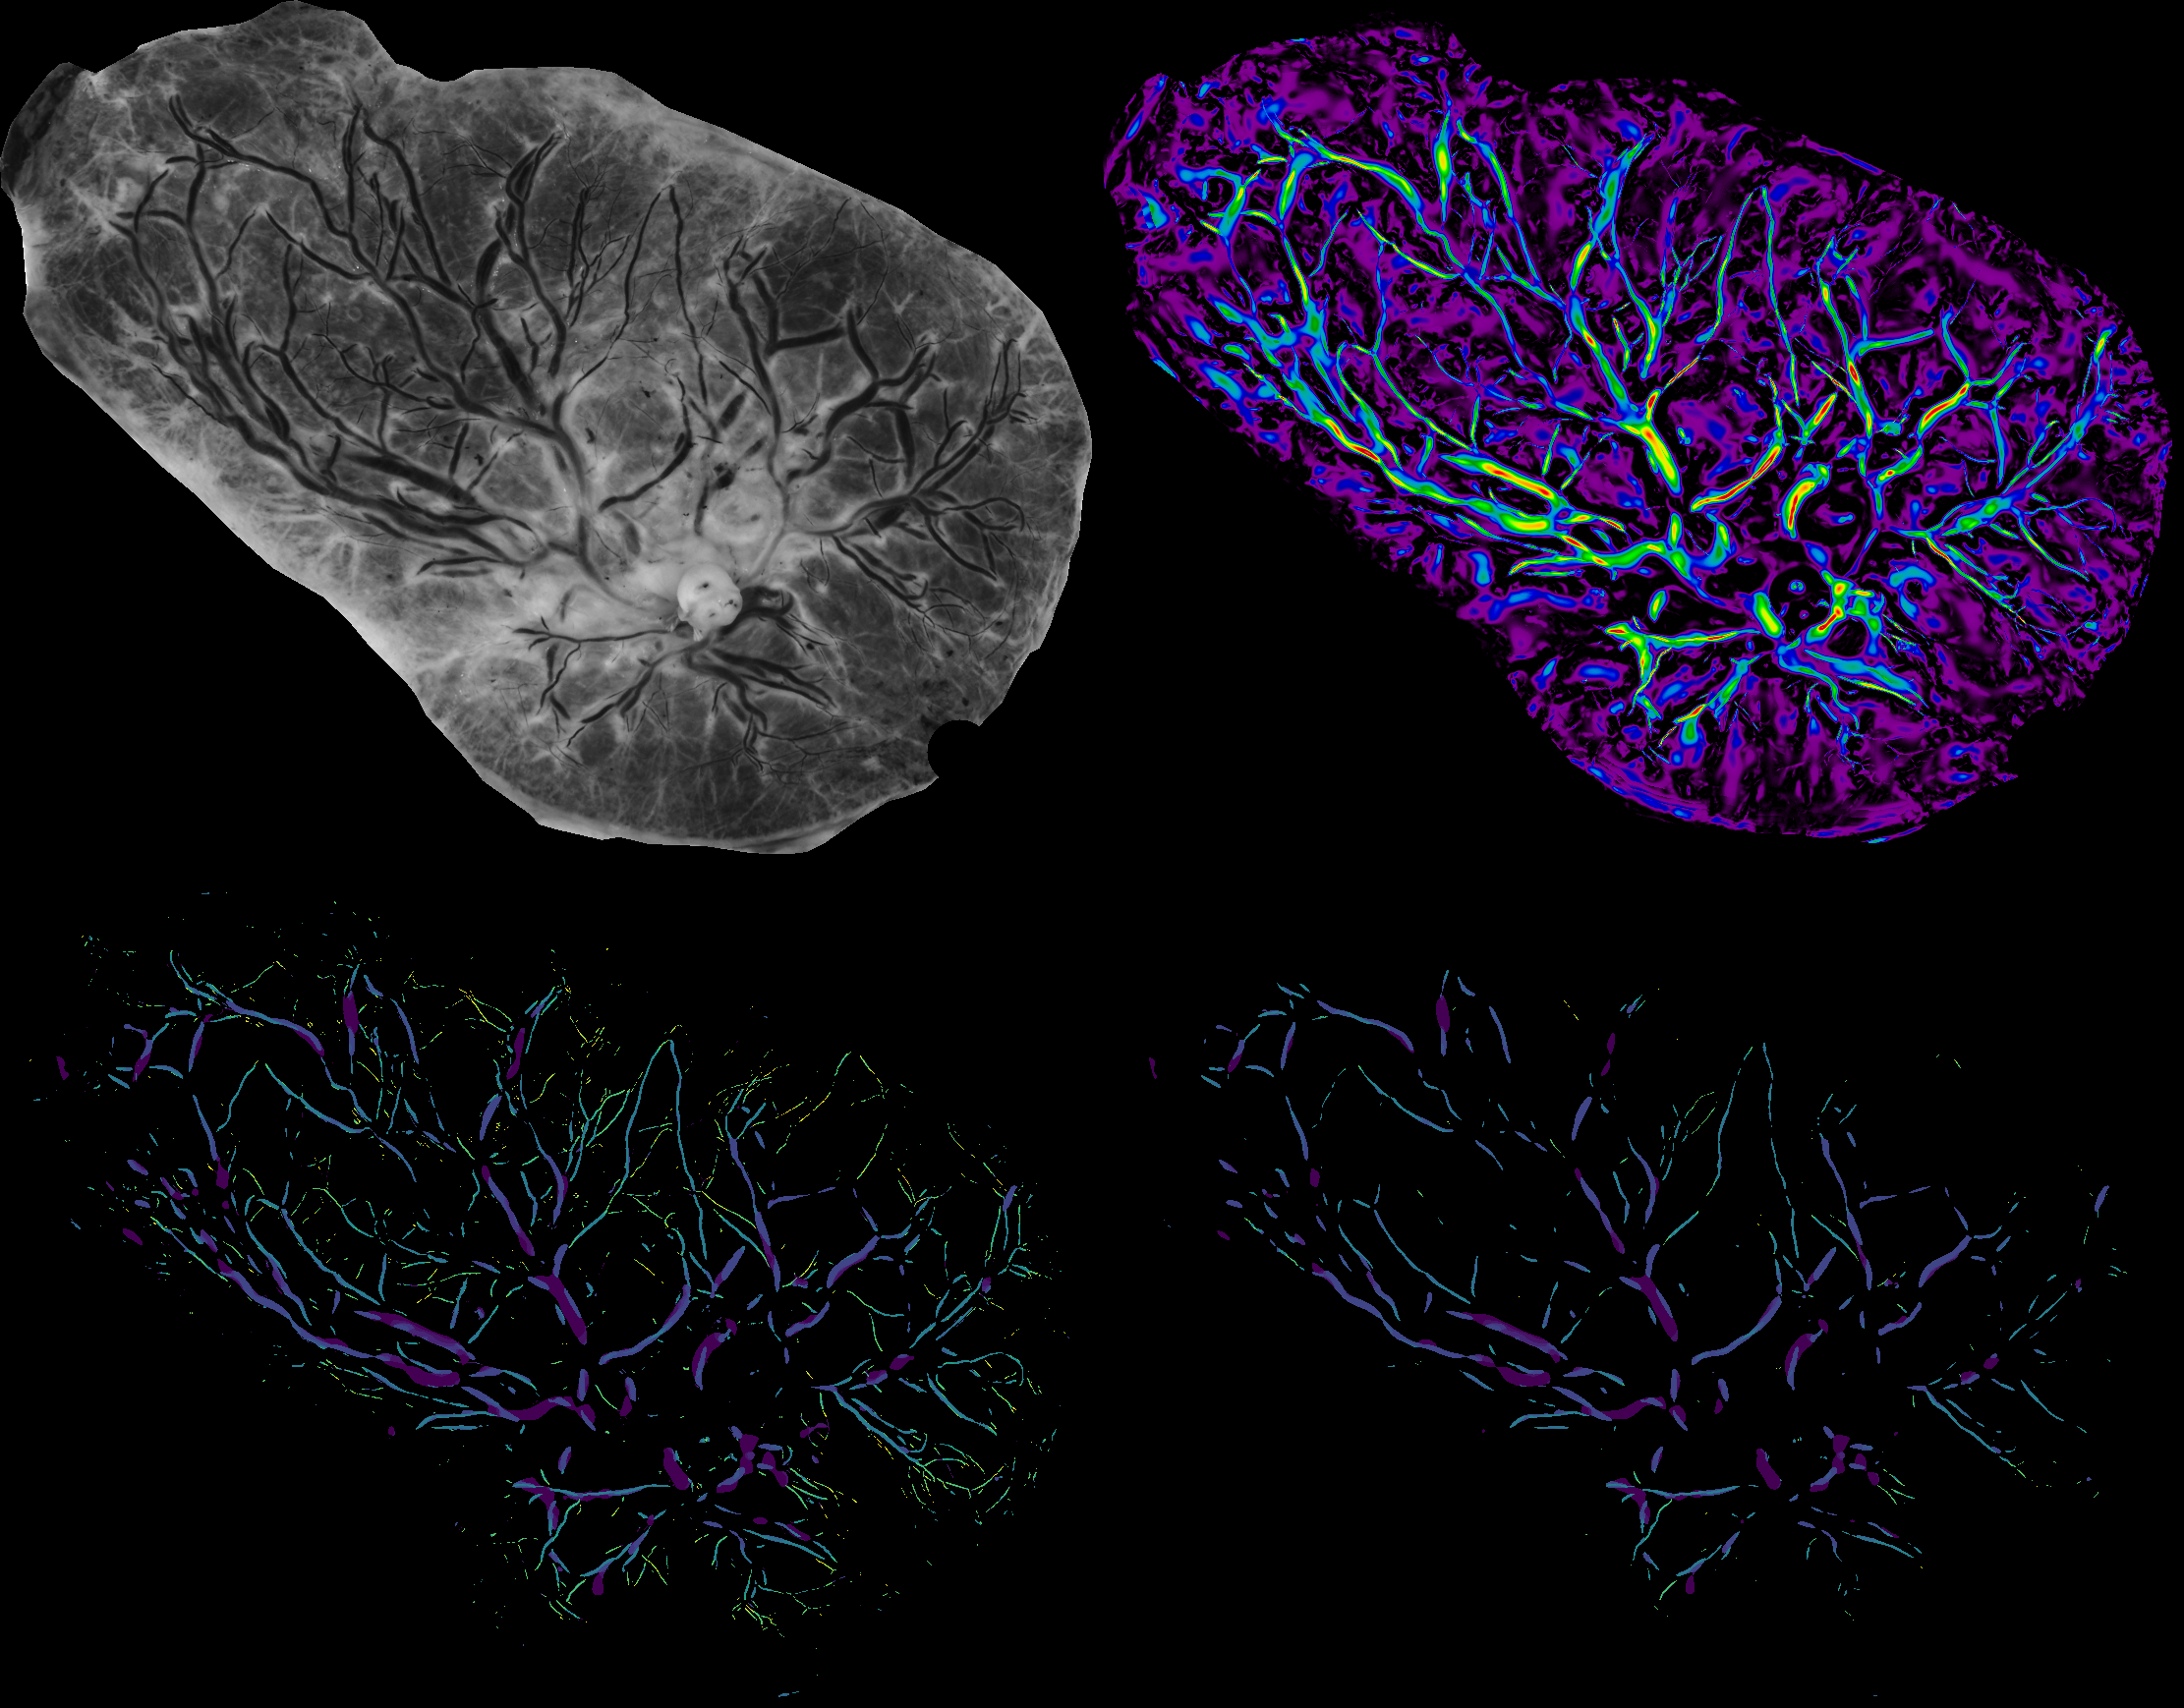
\includegraphics[width=\textwidth]{montage-T-BN0164923}
  \caption{Sample Multiscale Frangi output ($\beta=0.35$) with simple segmentation strategies (Example 1)}
  \label{fig:output-montage-example1}
\end{figure}

\begin{figure} \centering
  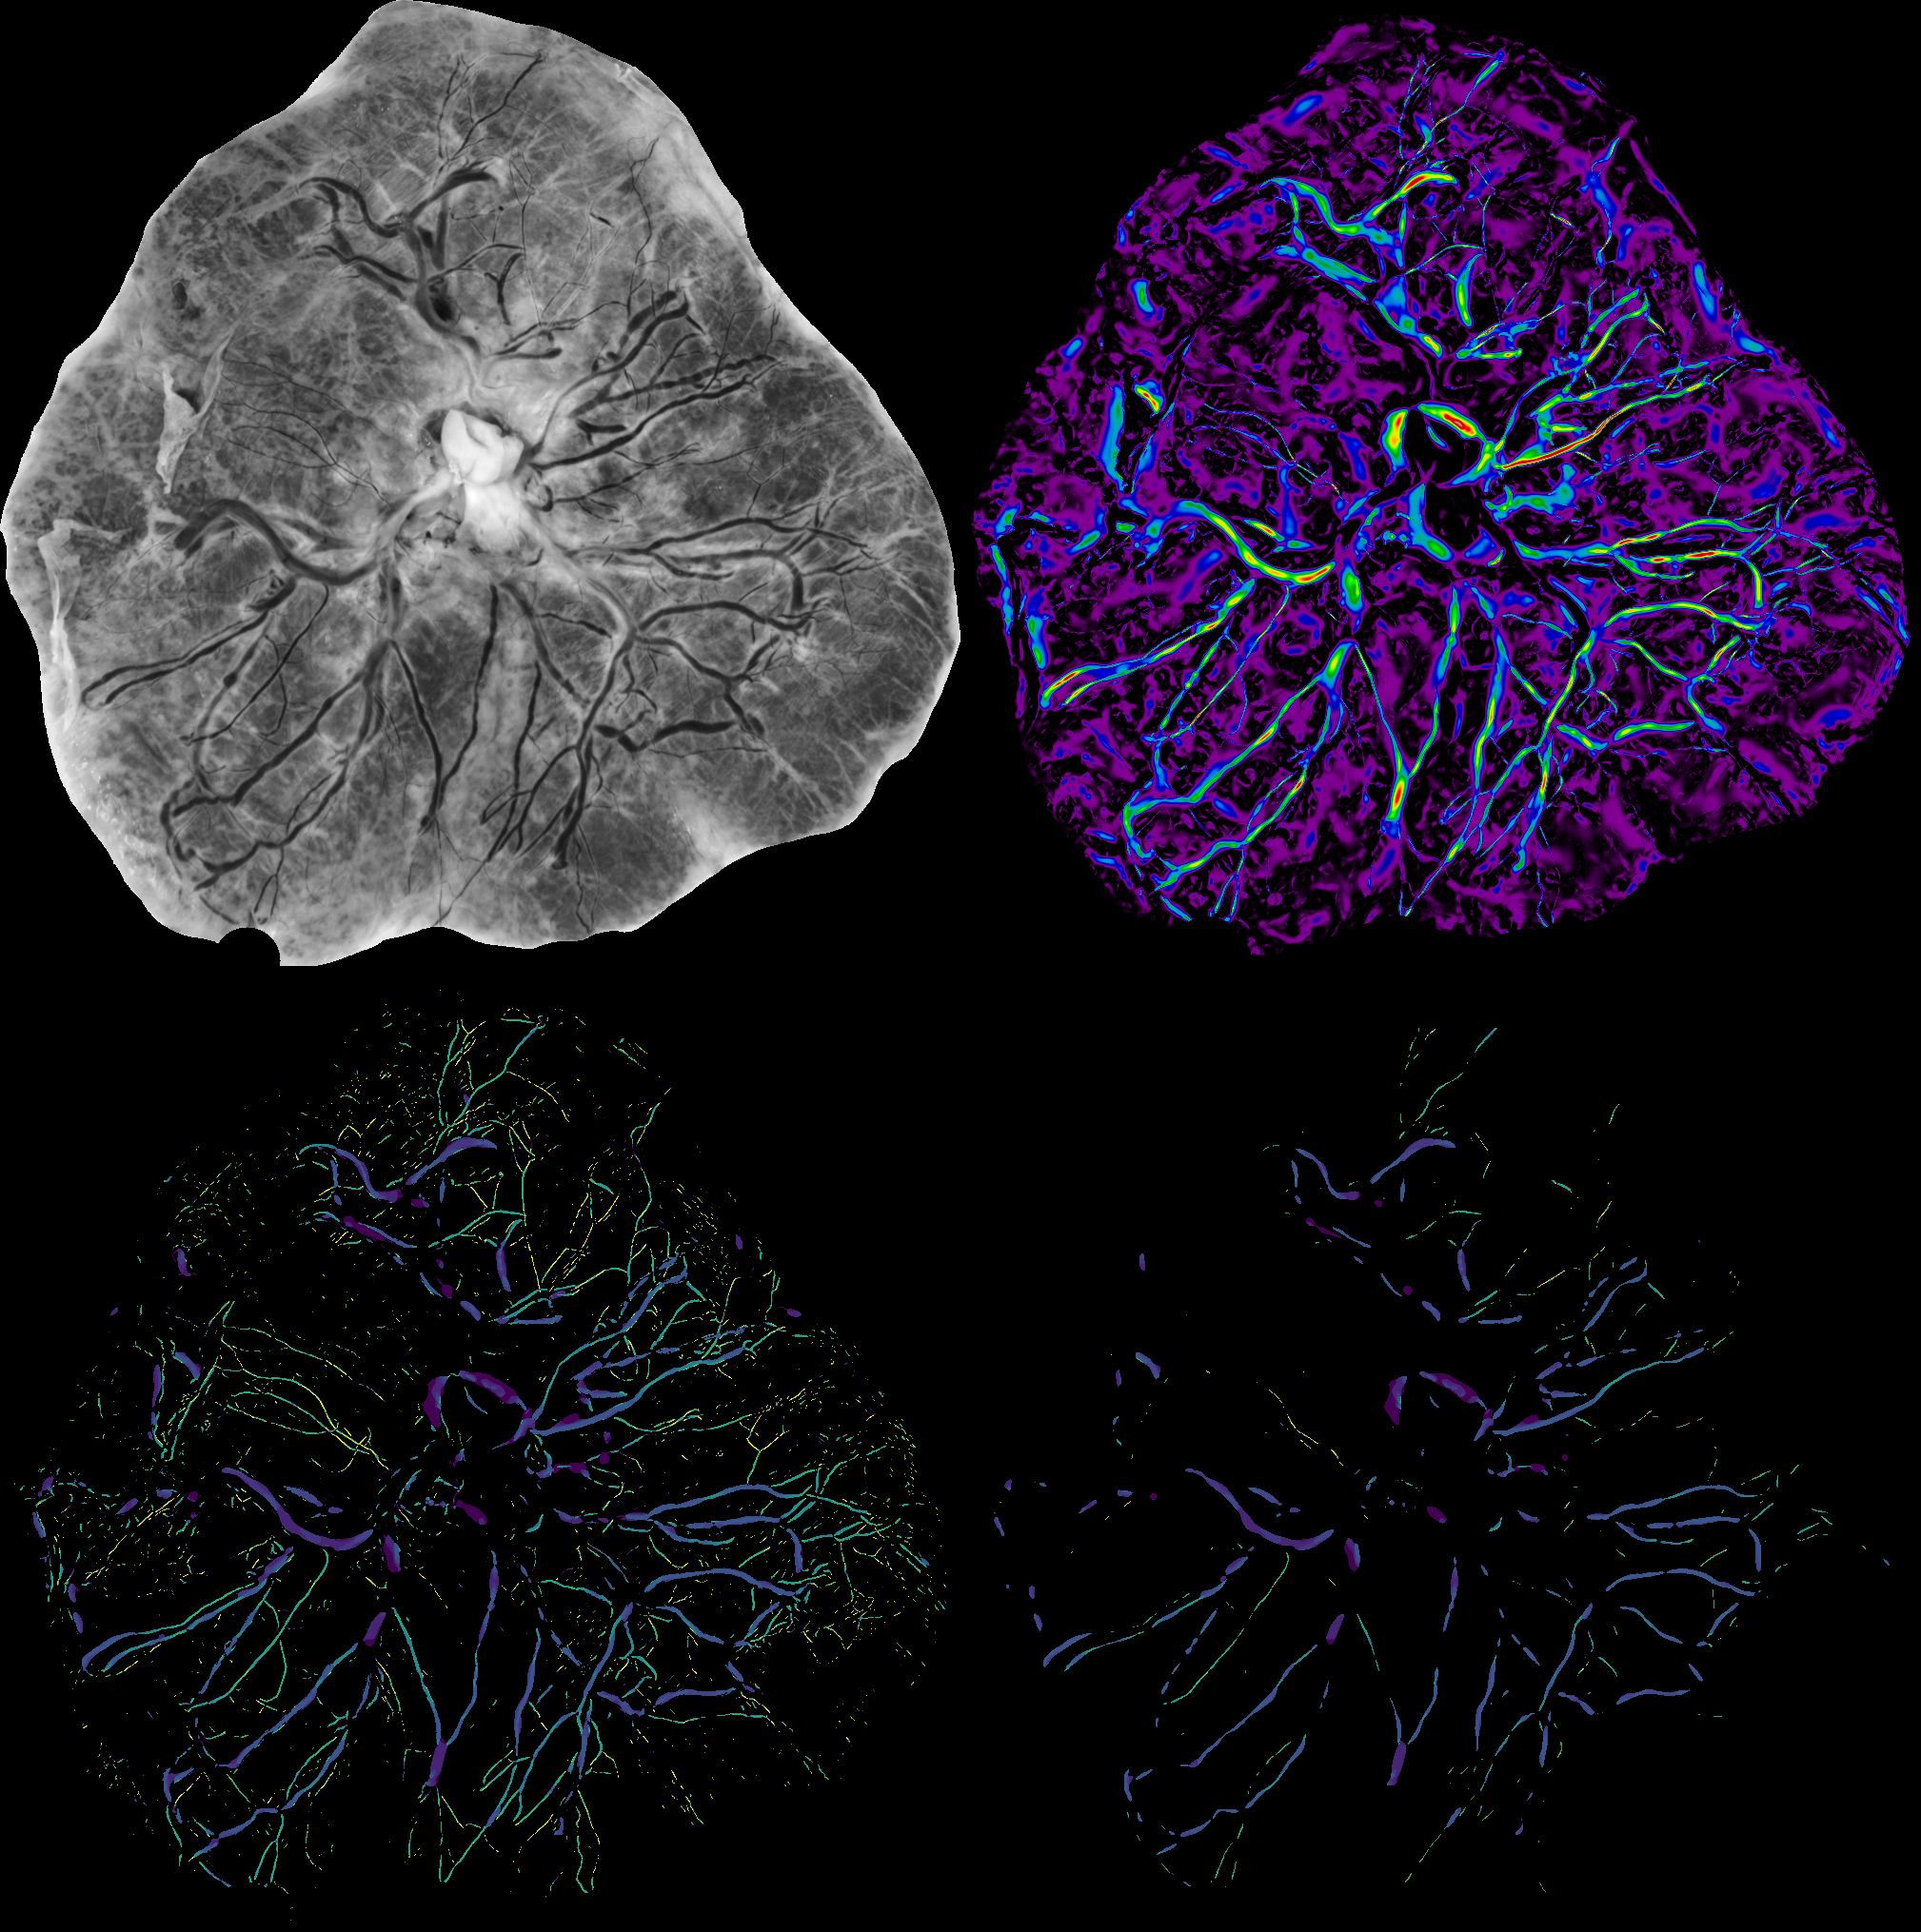
\includegraphics[width=\textwidth]{montage-T-BN0651415}
  \caption{Sample Multiscale Frangi output ($\beta=0.35$) with simple segmentation strategies (Example 2)}
  \label{fig:output-montage-example2}
\end{figure}


\begin{figure}
	\begin{minipage}[tp]{0.5\textwidth}
		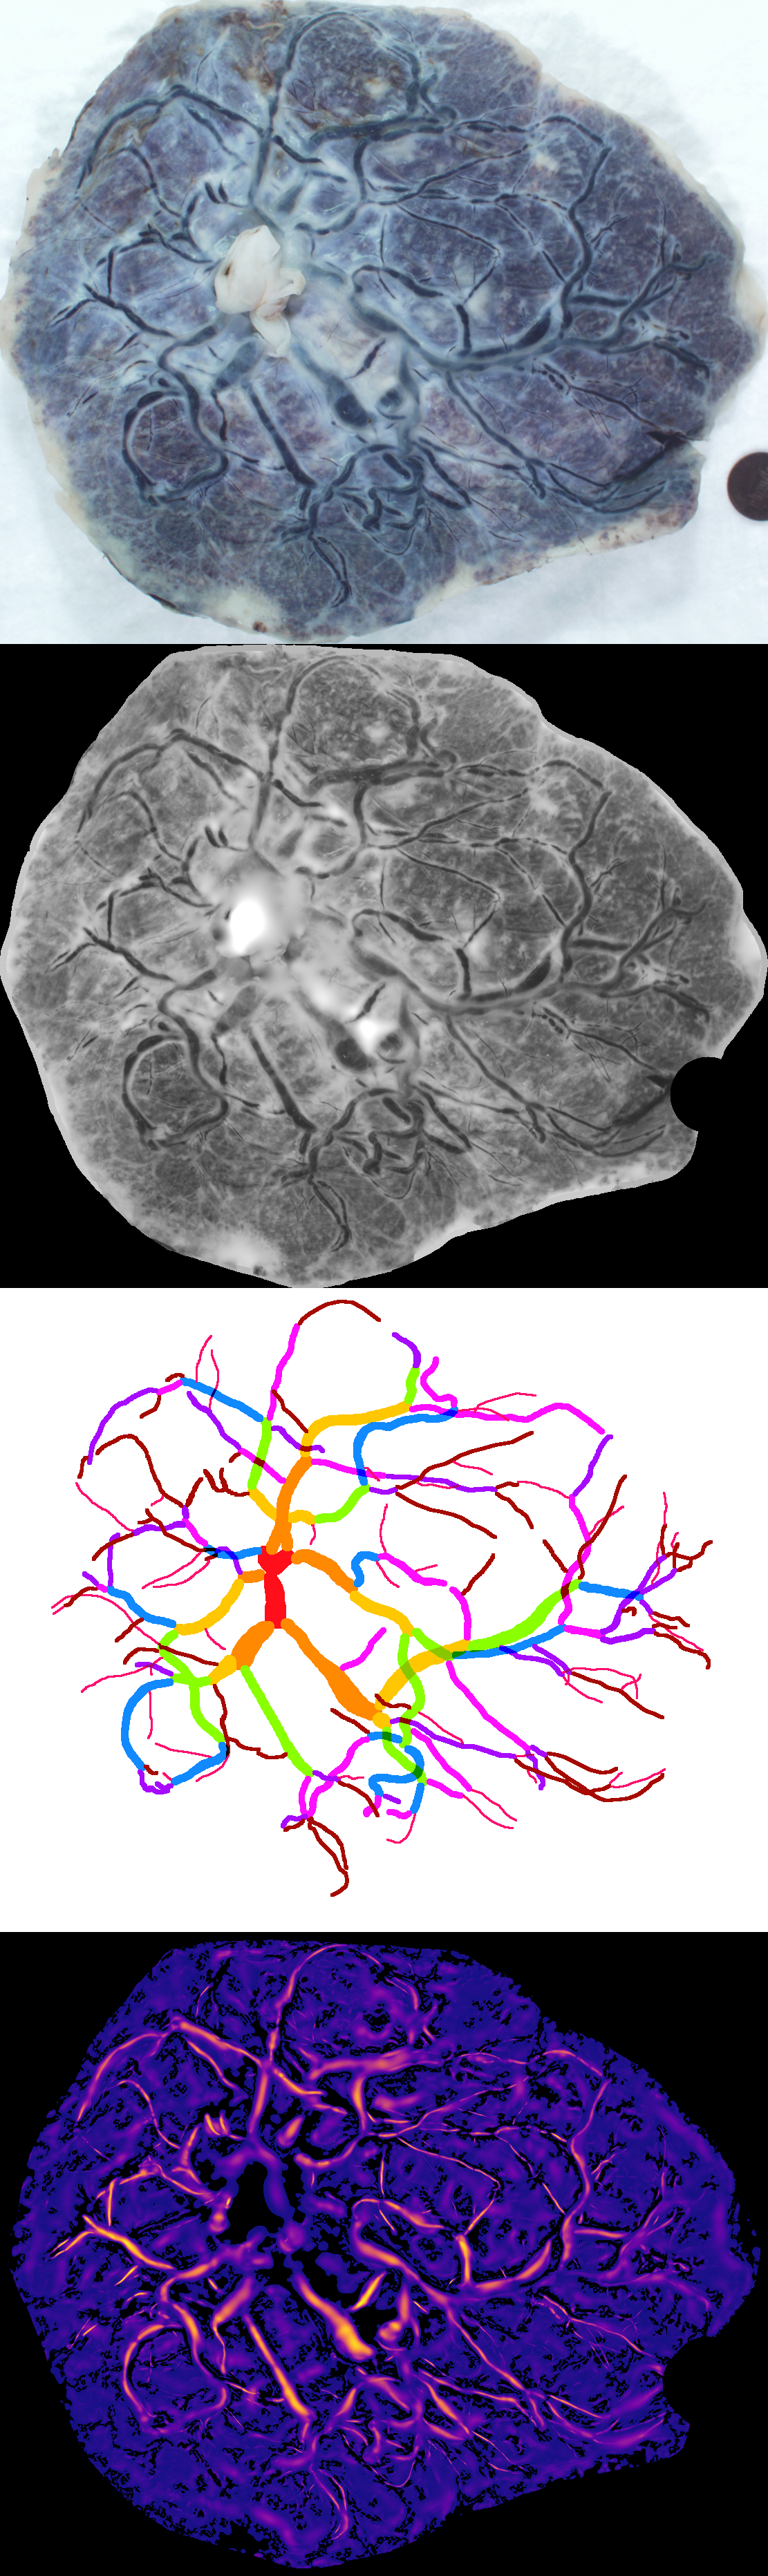
\includegraphics[height=0.95\textheight]{M1-T-BN2050224}
	\end{minipage}
	\quad
	\begin{minipage}[tp]{0.35\textwidth}
		\begin{tabular}{l|r|r|r}
			n  & $\sigma_n$  &  $\alpha_p$  &  $\max(V_\sigma)$ \\
			\hline
			0  &   0.3535 &  0.0547 &  0.986\\
			1  &   0.4243 &  0.0590 &  0.979\\
			2  &   0.5092 &  0.0654 &  0.970\\
			3  &   0.6110 &  0.0765 &  0.973\\
			4  &   0.7333 &  0.0892 &  0.988\\
			5  &   0.8801 &  0.0962 &  0.991\\
			6  &   1.0562 &  0.1082 &  0.991\\
			7  &   1.2676 &  0.1308 &  0.970\\
			8  &   1.5212 &  0.1669 &  0.973\\
			9  &   1.8256 &  0.2232 &  0.978\\
			10 &   2.1909 &  0.2925 &  0.984\\
			11 &   2.6294 &  0.3196 &  0.968\\
			12 &   3.1555 &  0.3269 &  0.994\\
			13 &   3.7869 &  0.3558 &  0.998\\
			14 &   4.5447 &  0.4058 &  0.999\\
			15 &   5.4542 &  0.3764 &  0.963\\
			16 &   6.5456 &  0.3184 &  0.950\\
			17 &   7.8553 &  0.3047 &  0.958\\
			18 &   9.4272 &  0.3287 &  0.916\\
			19 &  11.3137 &  0.3524 &  0.916\\
		\end{tabular} \\
	\end{minipage}
	\caption{Vesselness scores and percentile thresholds}
\end{figure}

\begin{figure}[p] \centering
	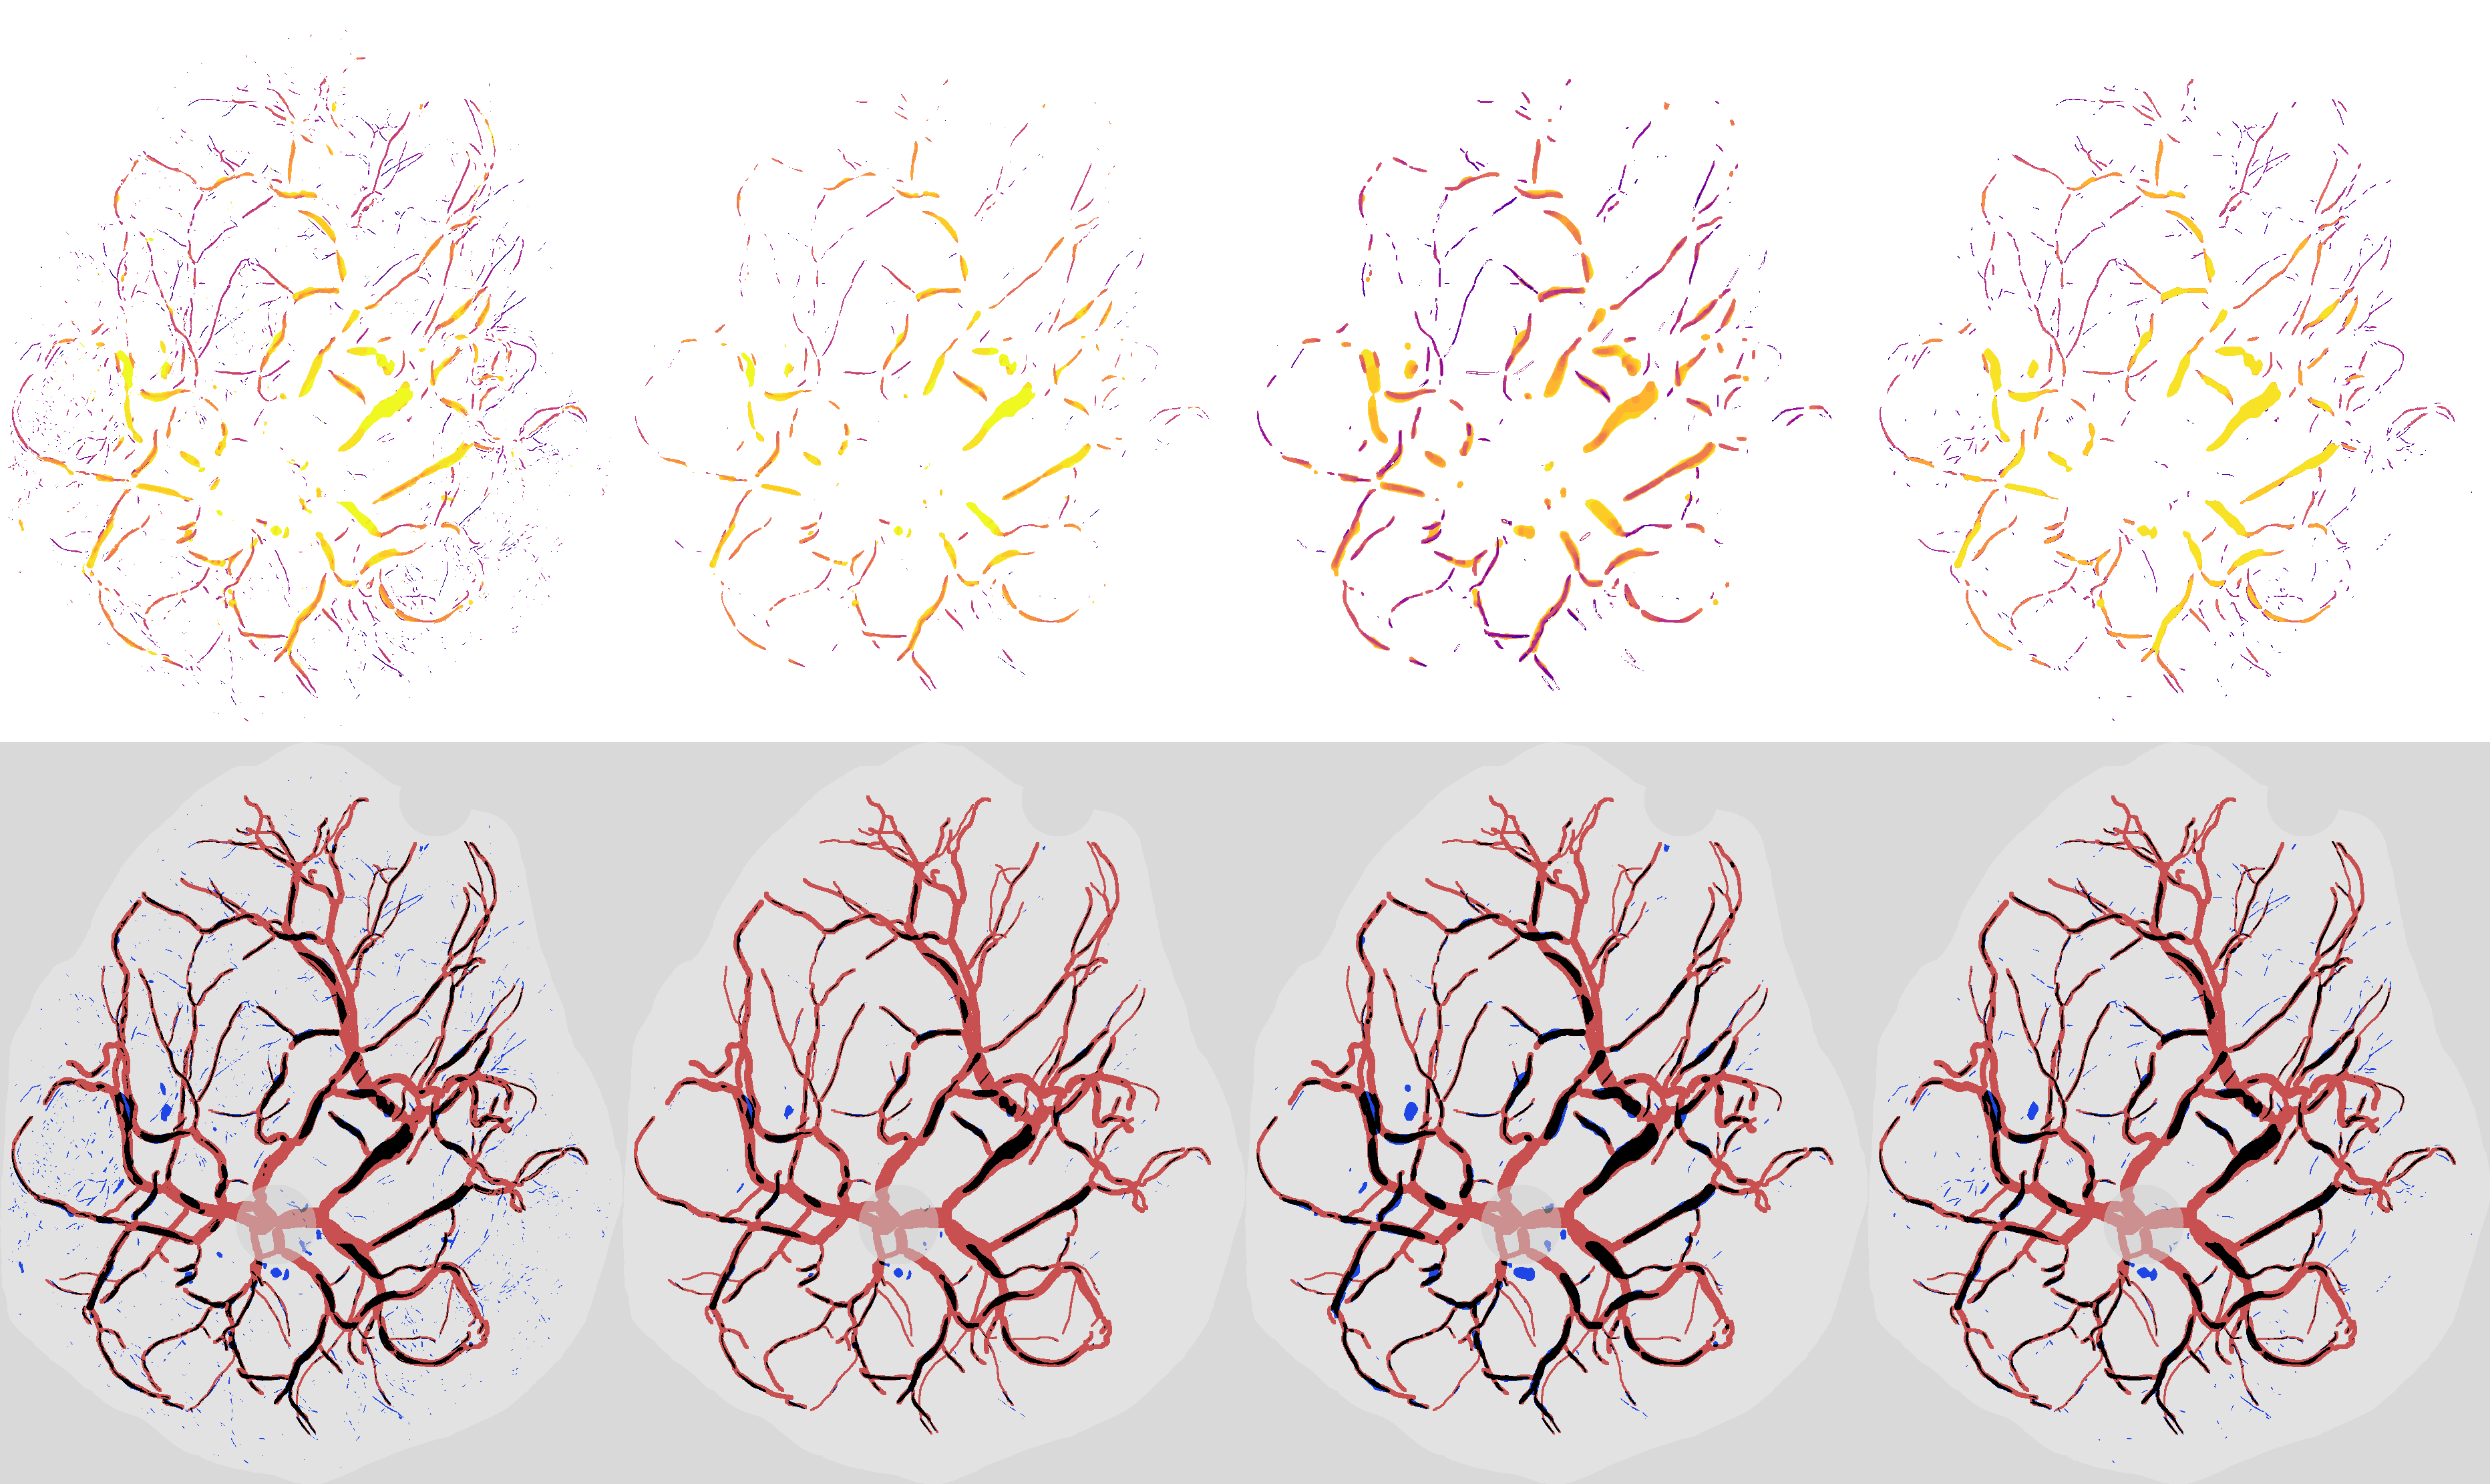
\includegraphics[width=\linewidth]{M2-T-BN2050224}
	\caption{Sample of Frangi-based Segmentation Methods (pt. 2)}
\end{figure}

%\begin{table}[p]\centering
%	\begin{tabular}{l|rrrr}
%		{} &        PF &        FA &        RW &        PS \\
%		\hline
%		MCC           &  0.4872 &  0.4208 &  0.5249 &  0.4877 \\
%		%\hline
%		skel coverage &  0.5085 &  0.3245 &  0.4493 &  0.4650 \\
%		%\hline
%		precision     &  0.8044 &  0.9472 &  0.8858 &  0.8697 \\
%	\end{tabular}
%	\caption{Scores for merging techniques}
%\end{table}:

\section{Variations in the Data Set and Imperfections of the Ground Truth} \label{sec:NCS-dataset-issues}
\begin{sidewaysfigure}
	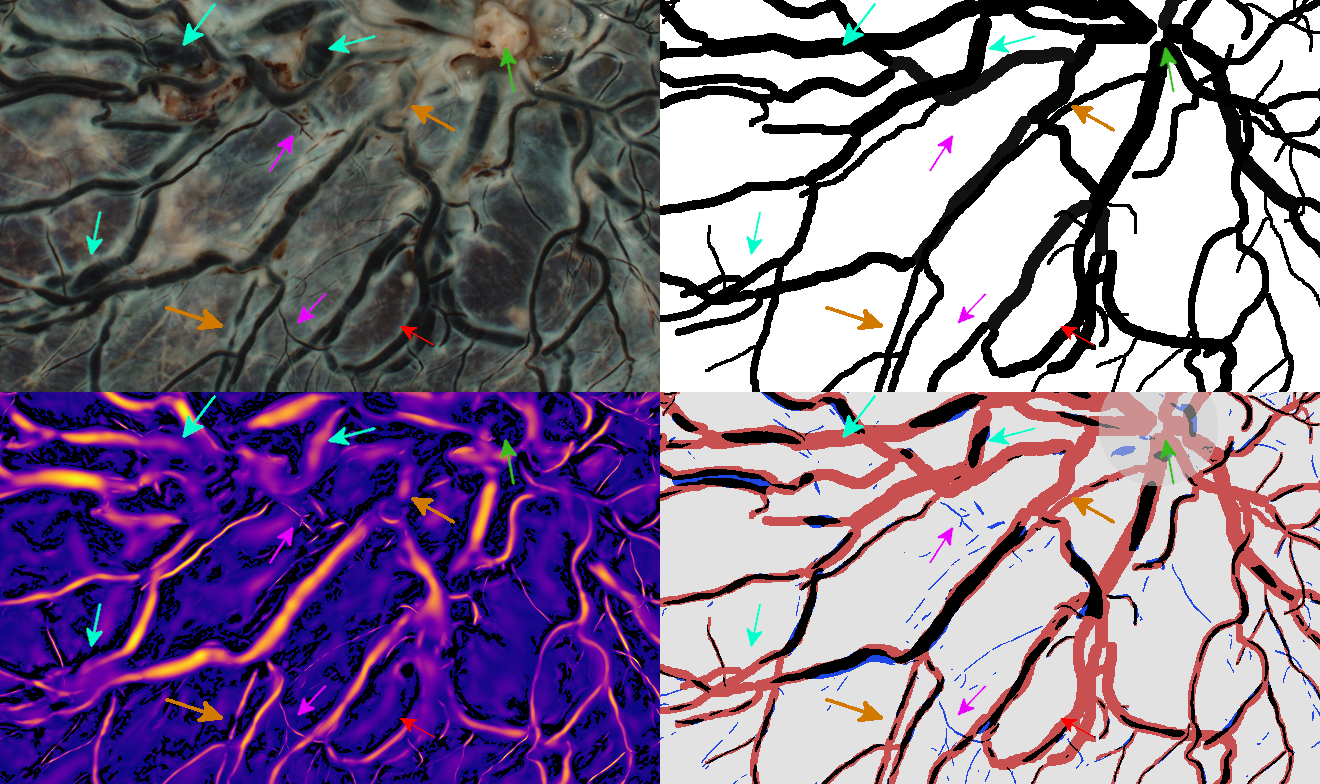
\includegraphics[width=\textwidth]{annotations-montage-2by2}
	\caption{Issues with the ground truth manifesting in Frangi vesselness scores}
	\label{fig:annotated-montage}
\end{sidewaysfigure}

We must qualify our binary classification. There are limitations intrinsic to the image domain and tracing protocol that make our ground truth tracing somewhat inaccurate. In \cref{fig:annotated-montage} we demonstrate a few common issues with the samples. The four figures show (top left) the original colored raw sample, (top right) the ground truth tracing, (bottom left) \Vmax, and (bottom right) the confusion matrix after some segmentation strategy. %"sieving strategy."
The green arrow points to the umbilical stump. You can see there is circular noise around this point, and in general perfusion around this point is very low--many of these vessels have been estimated by the tracer. The orange arrows represent points where perfusion is very low, perhaps caused by a clot in the blood vessel. The pink arrows point to vessels that were not traced, although they are clearly visible. The blue arrows point to where the shape of the vessel and the trace clearly do not agree. There any many more examples of these in the frame, and many more across all samples.

The red arrow points to an issue unrelated to the ground truth, but an issue that arise when selecting scales in our multiscale methodology-- this is a point of dark curvature that represents noise at larger scales. As you can see from the \Vmax of this inset, there is a positive response in this dead space between vessels, and there is another one that appears in the bottom left between two close vessels of similar size. 

\begin{figure} \centering
  \subfloat{
  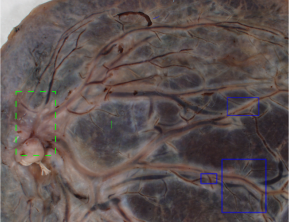
\includegraphics[width=0.5\textwidth]{T-BN0392644_inset}
}
\subfloat{
  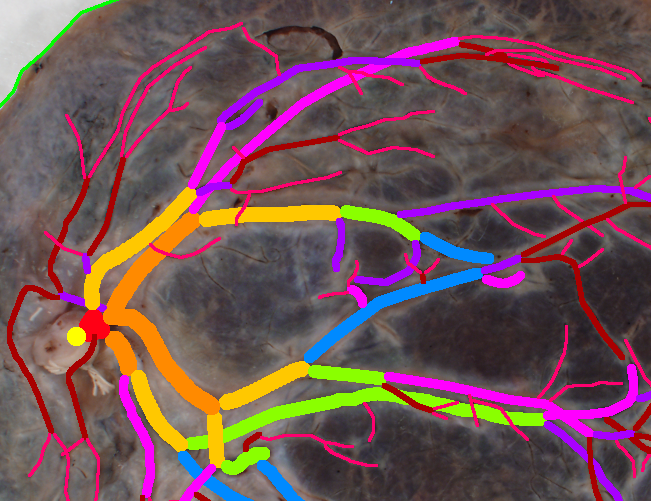
\includegraphics[width=0.5\textwidth]{T-BN0392644_inset_ctrace}
} \\
\subfloat{
  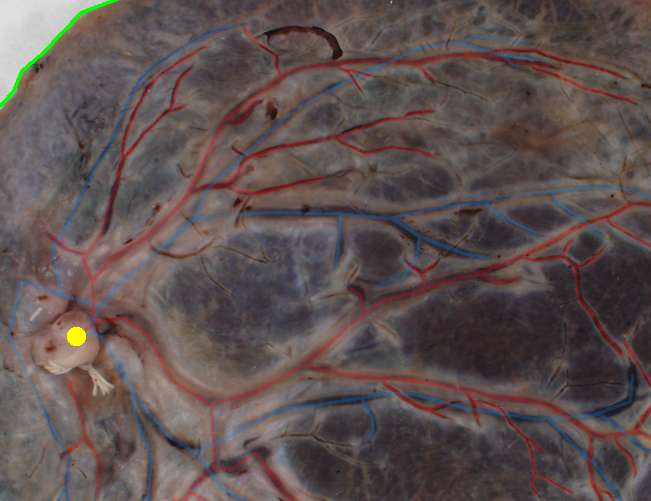
\includegraphics[width=0.5\textwidth]{T-BN0392644_inset_sketches}
}
\subfloat{
  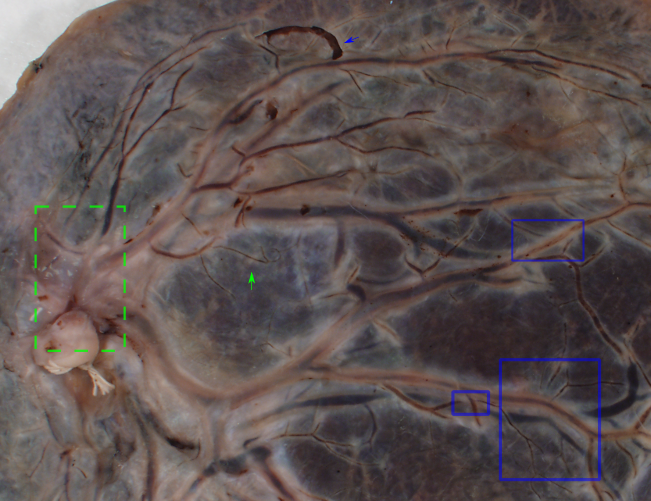
\includegraphics[width=0.5\textwidth]{T-BN0392644_inset_mark}
}
\caption{Issues with ground truth and sample quality}
\label{fig:groundtruth-samplequality}
\end{figure}

As seen in \cref{fig:groundtruth-samplequality}, there are several issues with the samples that will cause trouble in our efforts toward segmentation. Our represenative sample is BN0392644. The top left is the original (color) image, the top right is the full vessel width trace. The bottom left is a smaller skeletonization (sketch), where arteries are shown in red and veins are shown in blue. The bottom right figure contains some annotations. At the top, a blue arrow indicates a large curvilinear patch of dried blood that is not part of the vascular network. The green arrow in the middle indicates some vessels that are too small for the diameter binning and are thus not reported. We will see later that our Frangi result perfectly captures these, yet they will be reported as a false positive since they are not part of the tracing. However, there are other vessels of similar visual width in this same inset that are traced. In blue boxes (and in many other spots) the vessels cross each other. The border around these will prevent us from being able to extract the vessel directly. In the green dotted box, a major arterial and a major venous branch each connect to the umbilical cord insertion point. Whereas the arterial branch (on the right) can be seen, it will not be reported by the Frangi filter, since those points are not darker relative to the background. You can also see how much variation there is as you look along a blood vessel. There are some areas where the Frangi filter will have a very limited response. 



\begin{enumerate}
\item Collar is stupid and should really be considered like a error in marking the perimeter. Throw these away or edit. Maybe make a section called discarded samples that's stupid but yeah.
\item Vessels suck sometimes. In the portion above, 1602443, there's a random blood clot which gets identified at large $\sigma$. But also the small forked shaped thing which is obviously a vessel doesn't get defined.
\item Too much blood (not enough?? no idea) is left in the vessels. leading to the weird white border around some vessels. you could identify these along with black center and combine them somehow. no idea.Also, holy shit, some of the white vessel ``sleeves'' ARE identified in the tracing, and some aren't. Find an example of this and whine about it.
\item Umbillical cord insertion point is stupid and obscures a lot. The tracer guesses but there's no real guiding principle AFAIK..
\item Small vessels aren't accounted for at all. Not sure how to coincide measurement in terms of scale space anymore, but should figure out how to cut off those values before running MCC metric.
\end{enumerate}

An example of bad samples that performed comparatively poorly across all segmentation methods can be found in the \cref{bad_gallery}. You can see that there is a lot of "noise" on the sample itself, and in some cases the vessels are much larger than other samples and therefore weren't picked up.

\begin{figure}[p]
	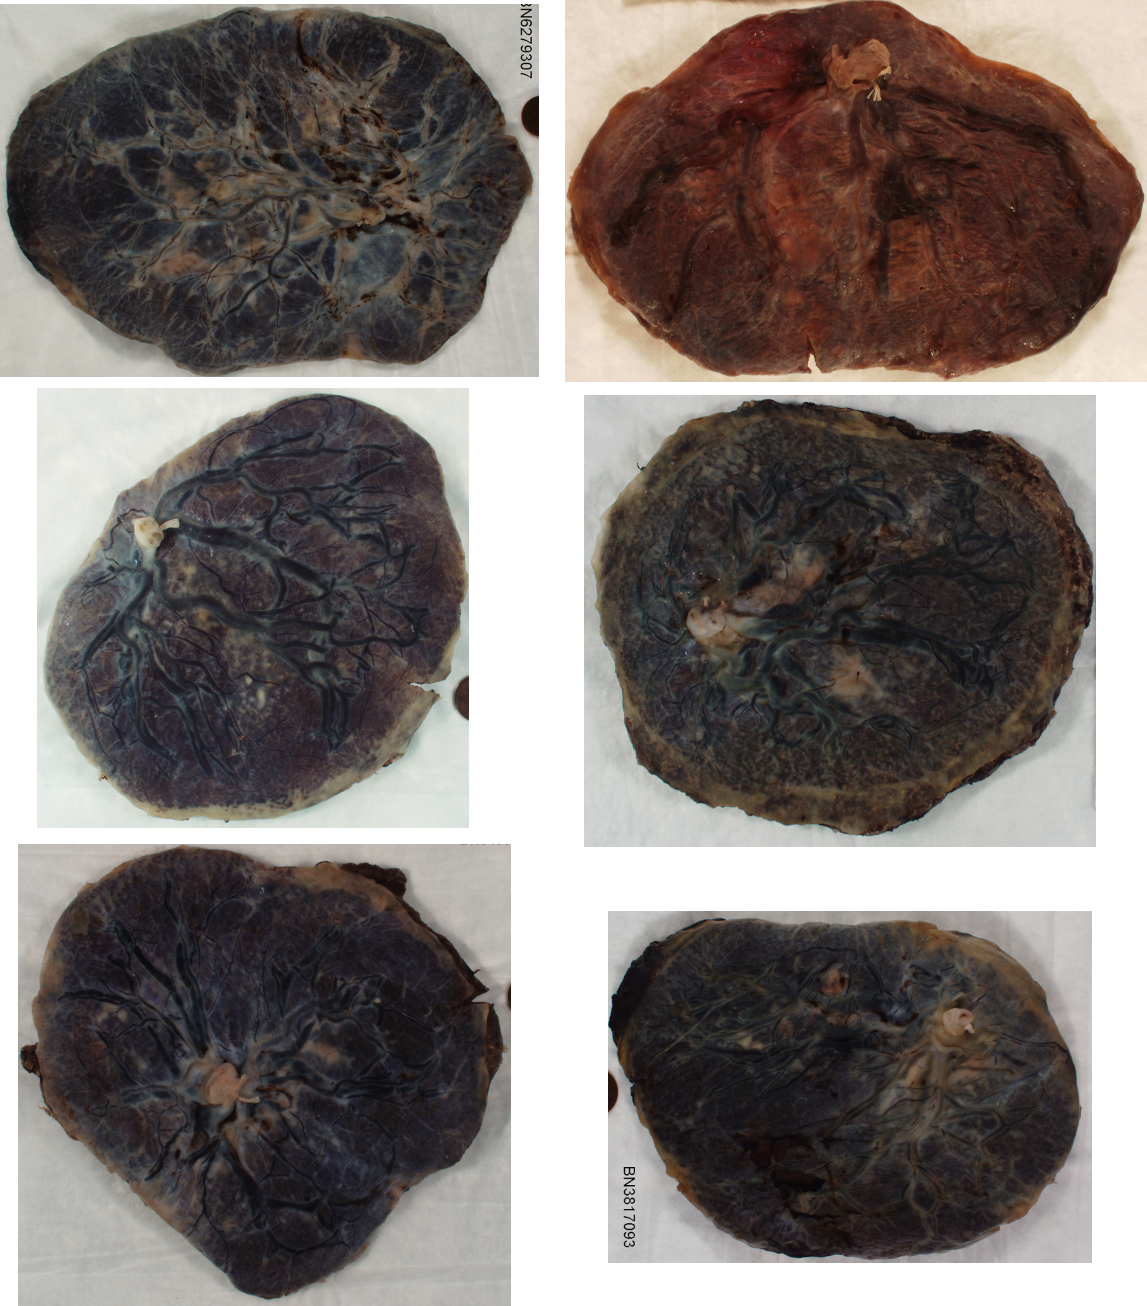
\includegraphics[width=\textwidth]{bad_gallery}
	\caption{Bad samples}
	\label{fig:bad-gallery}
\end{figure}

\section{Results}

In \cref{fig:compare_parameters}, we demonstrate the usefulness of scricter parameters for the Frangi filter. Since the Frangi vesselness measure is a "probability-like" score, we should be interested--without doing any actual segmentation yet--to what extent this score aligns with the ground truth in a cumulative sense. We should hope at least that larger values of We define the cumulative vesselness ratio by ``integrating'' the max vesselness score over pixels in the ground truth and over the entire image and considering the ratio:

\begin{defn} The cumulative vesselness ratio for a particular parametrization of the multiscale Frangi filter is given by
	\begin{equation}
	CVR\left(\Vmax\right) := \frac{\sum_{G\subset\img} \Vmax(x_0, y_0)}{\sum_{\img} \Vmax(x_0,y_0)}
	\end{equation}
	where the sums on top and bottom are being carried out for all pixels $(x_0,y_0)$ in the "ground truth" subset $G$ in the image $\img$
	and over the entire image $\img$ itself, respectively.
\end{defn}

\cref{fig:compare_parameters} shows $\Vmax$ for two well-behaved samples with reported $CVR$. We see in both cases that stricter parameters (smaller $\beta$ and larger $\gamma$) correspond to an increased $CVR$. Each of these sample was run over the same scales (logarithmically spaced from $2^{-1.5}$ to $2^{3.5}$ with $N=20$ and the color output of each $\Vmax$ is normalized between 0 and 1.

\begin{figure}[p]\centering
	\subfloat{
		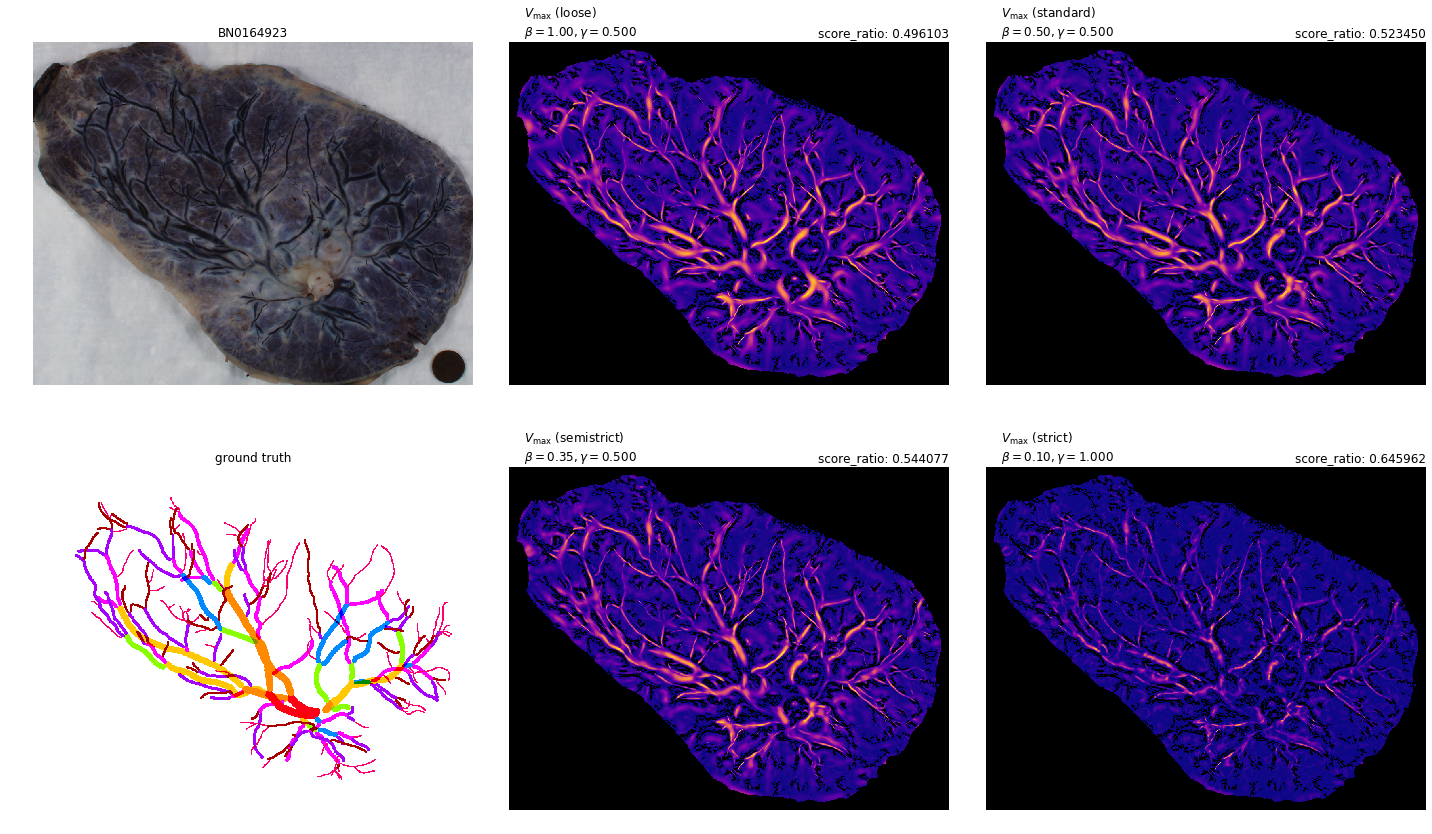
\includegraphics[width=\textwidth]{compare_parameters_BN0164923}
	}\\
	\subfloat{
		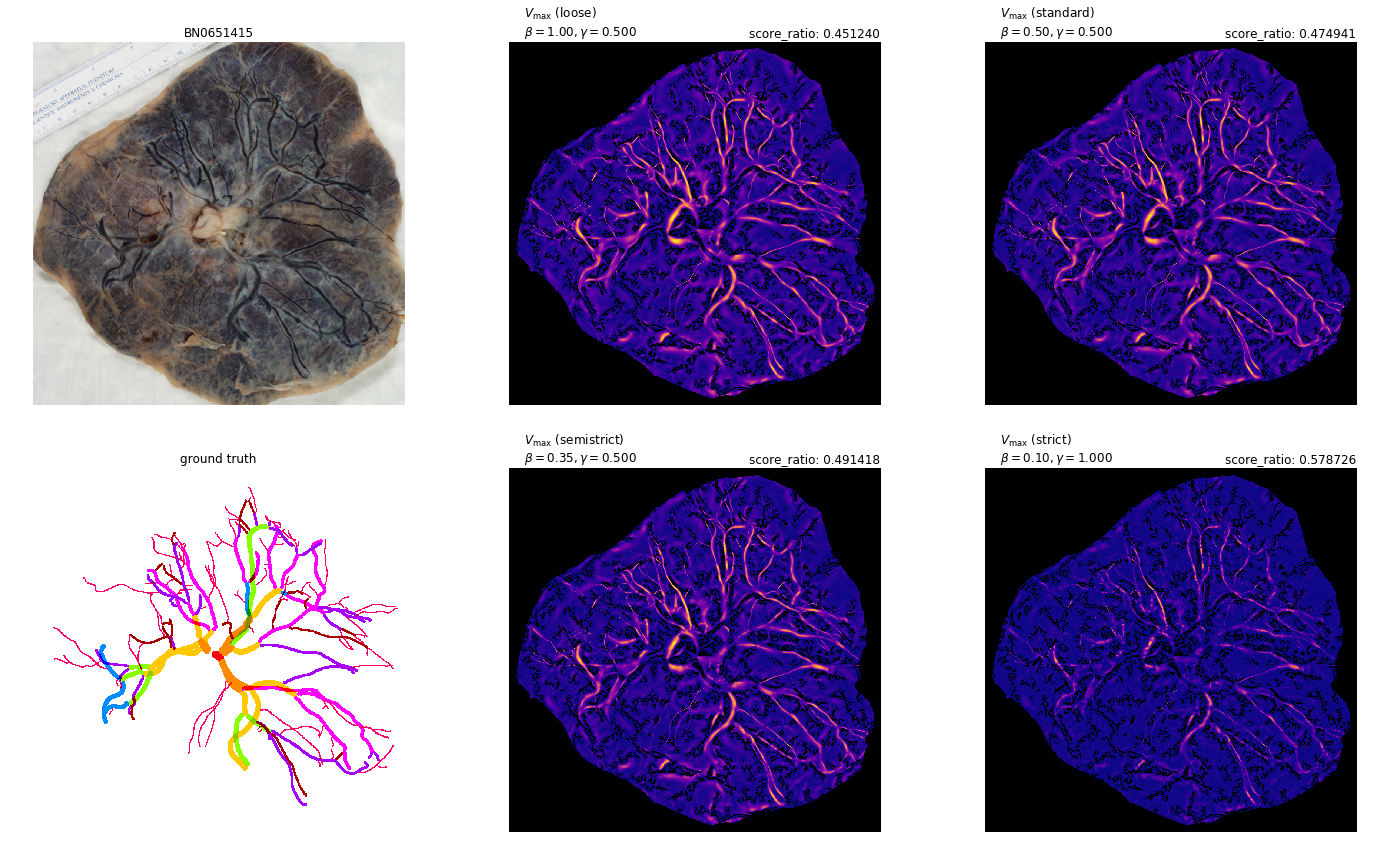
\includegraphics[width=\textwidth]{compare_parameters_BN0651415}
	}
	\caption{\Vmax  and $CVR$ for different parameter choices}
	\label{fig:compare_parameters}
\end{figure}

\begin{figure}[p]
  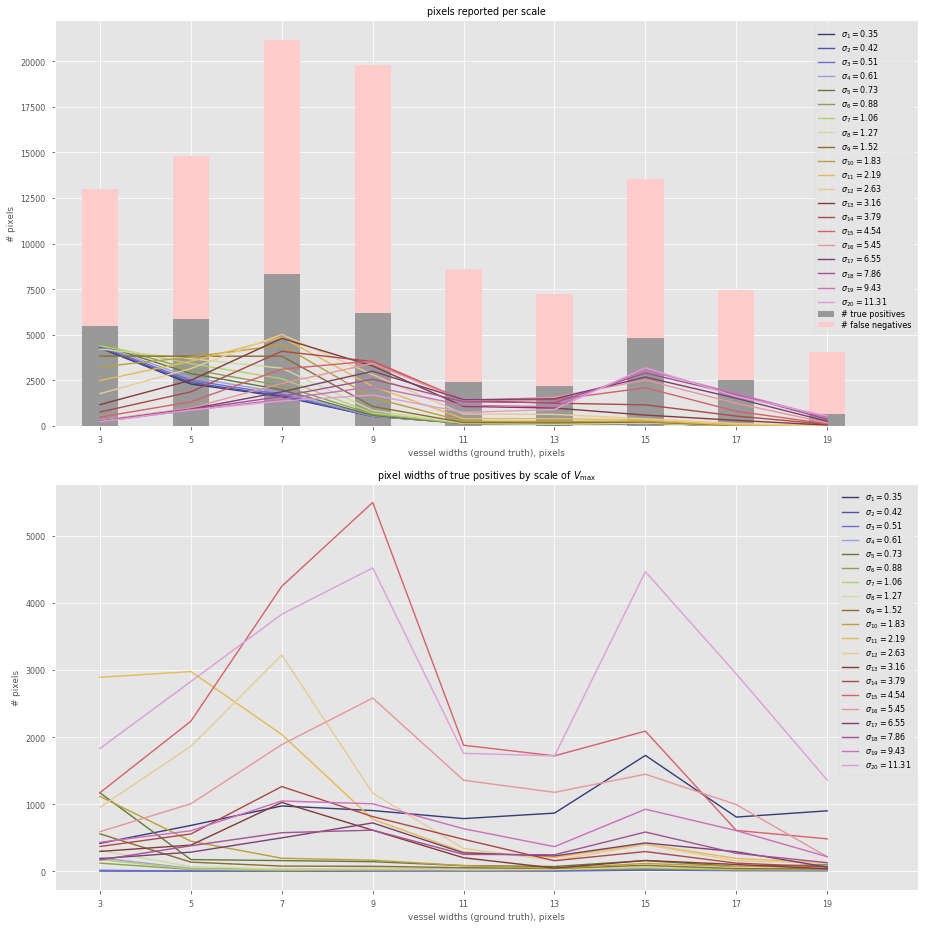
\includegraphics[width=\textwidth]{test-scale-width}
  \caption{Pixel Width of Ground Truth vs. Scale Length for True Positives}
\end{figure}

\begin{figure}[p]\centering
		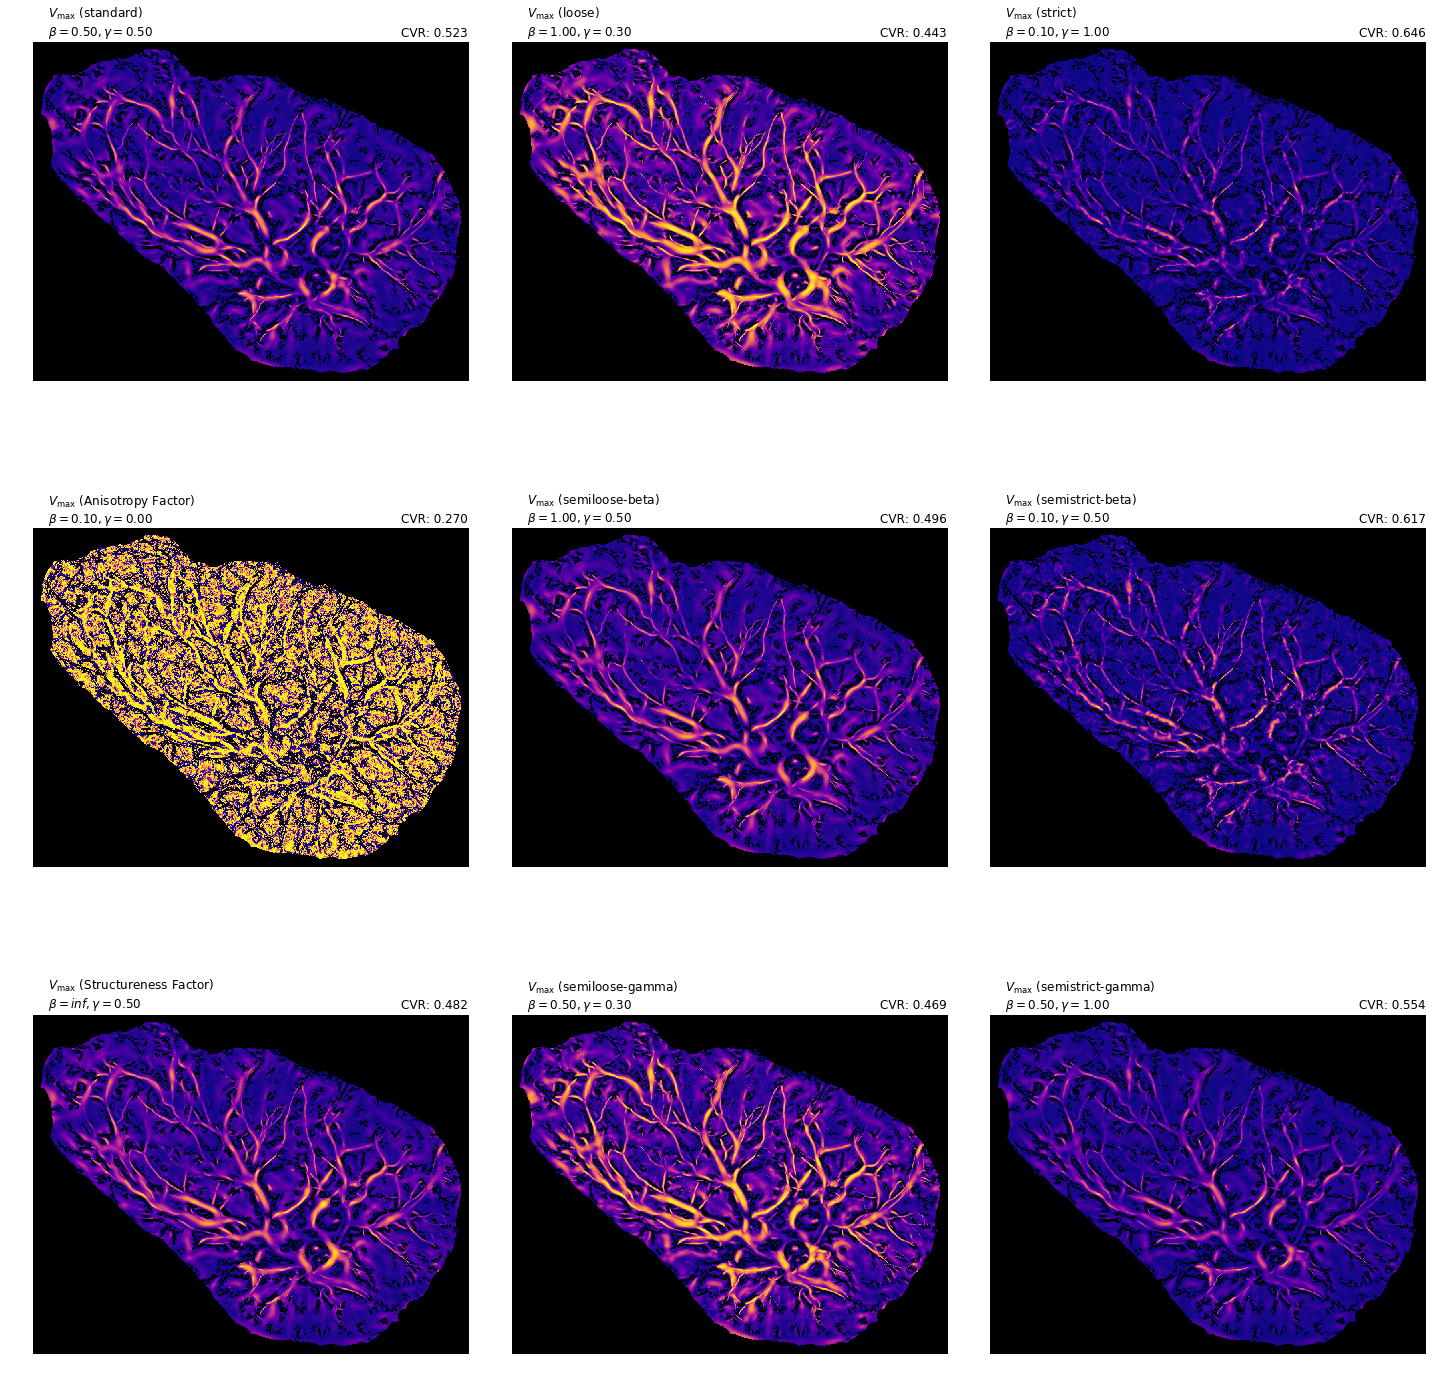
\includegraphics[width=\textwidth]{compare_parameters_3by3_example1}
	\caption{\Vmax  and $CVR$ for varying multiscale Frangi parametrizations (Example 1)}
	\label{fig:compare_parameters_3by3_example1}
\end{figure}

\begin{figure}[p]\centering
	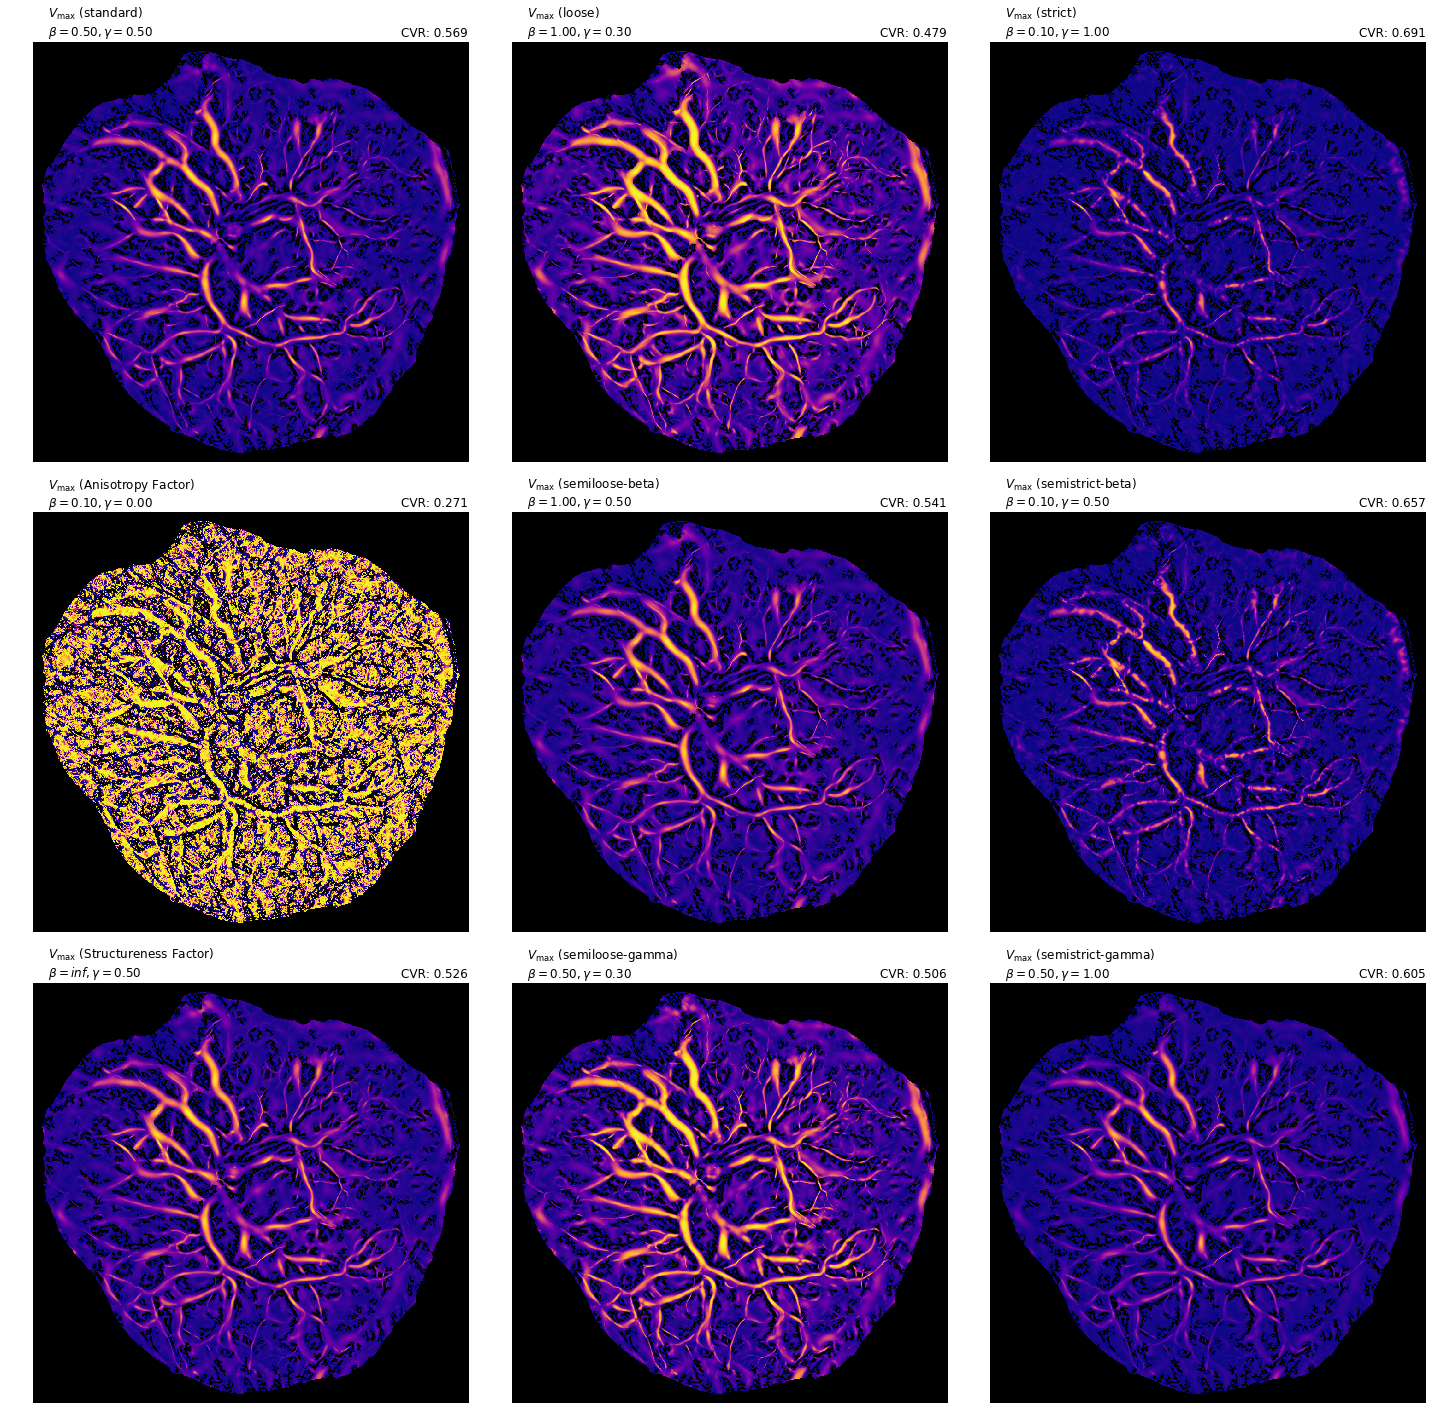
\includegraphics[width=\textwidth]{compare_parameters_3by3_example2}
	\caption{\Vmax  and $CVR$ for varying multiscale Frangi parametrizations (Example 2)}
	\label{fig:compare_parameters_3by3_example2}
\end{figure}

\begin{figure}\centering
	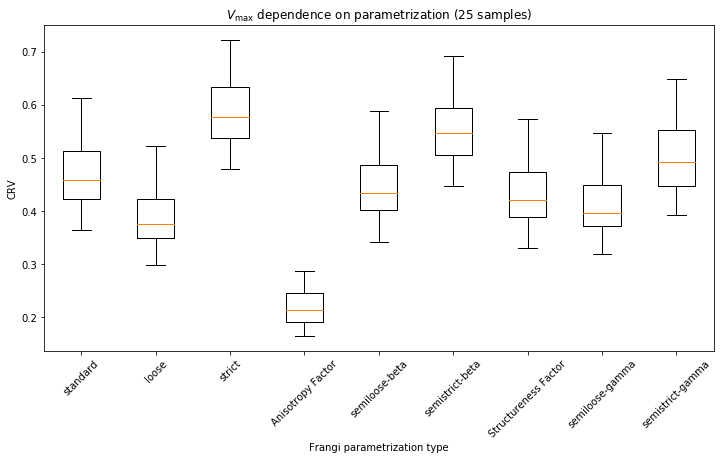
\includegraphics[width=\textwidth]{CRV_boxplot_quality0}
	\caption{$CVR$ scores of 25 samples under varying parametrizations}
  \label{fig:CVR-boxplot-quality0}
\end{figure}

In \cref{fig:CVR-boxplot-quality0} we show how the CVR is affected for 25 of the ``best'' samples, that is, those that generally fared better for segmentation techniques. This shows that the  results of \cref{fig:compare_parameters_3by3_example1} and \cref{fig:compare_parameters_3by3_example2} hold in general for all ``well-behaved'' samples in our image domain. 
\begin{figure}[p]\centering
  \subfloat{
  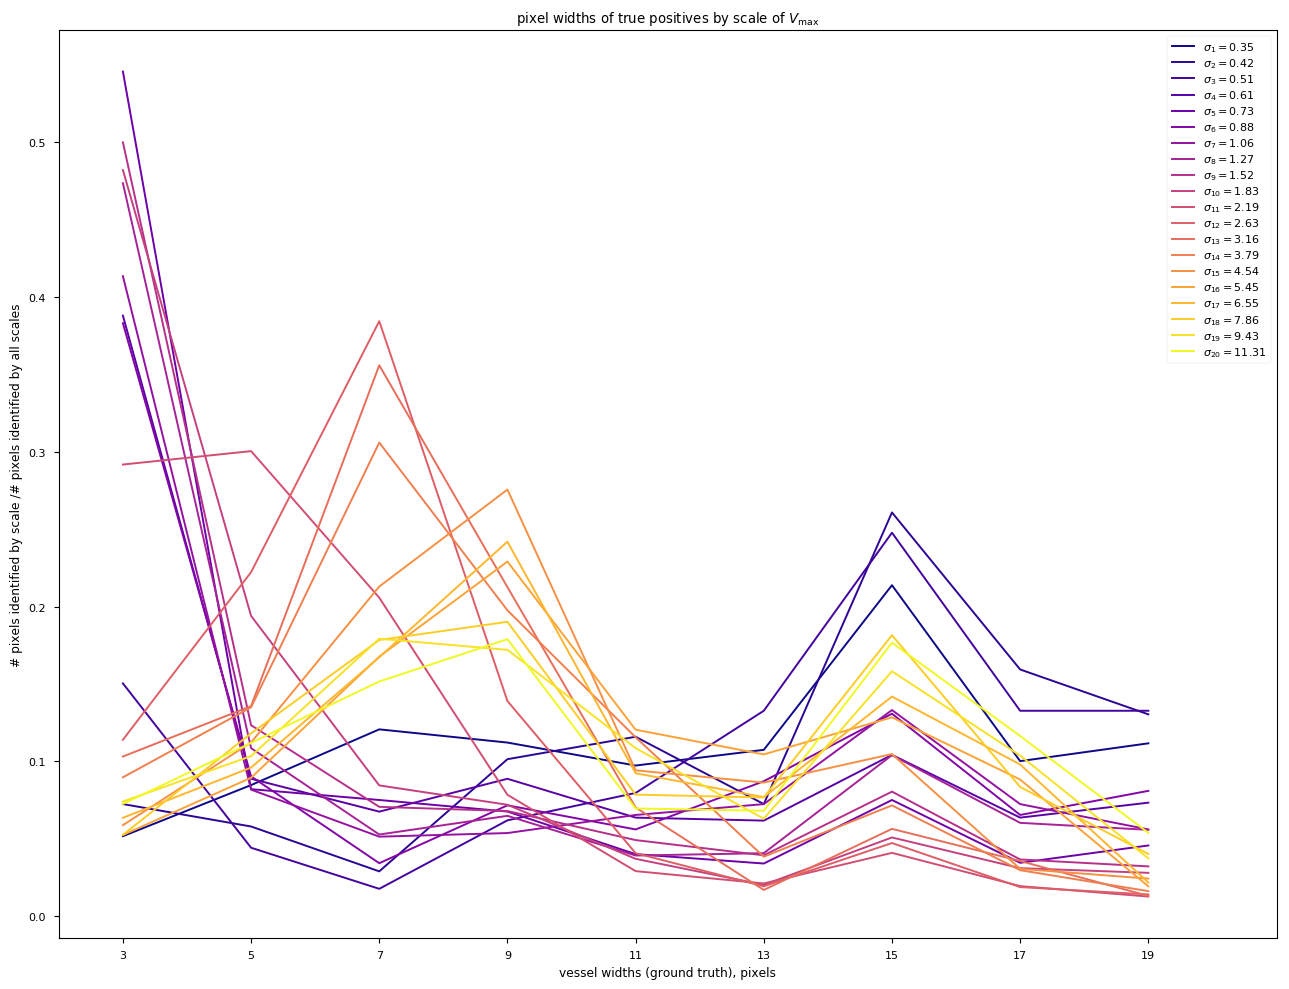
\includegraphics[width=0.85\textwidth]{Vmax_to_scale_normalized}
  }\\[-0.5cm]
  \subfloat{
  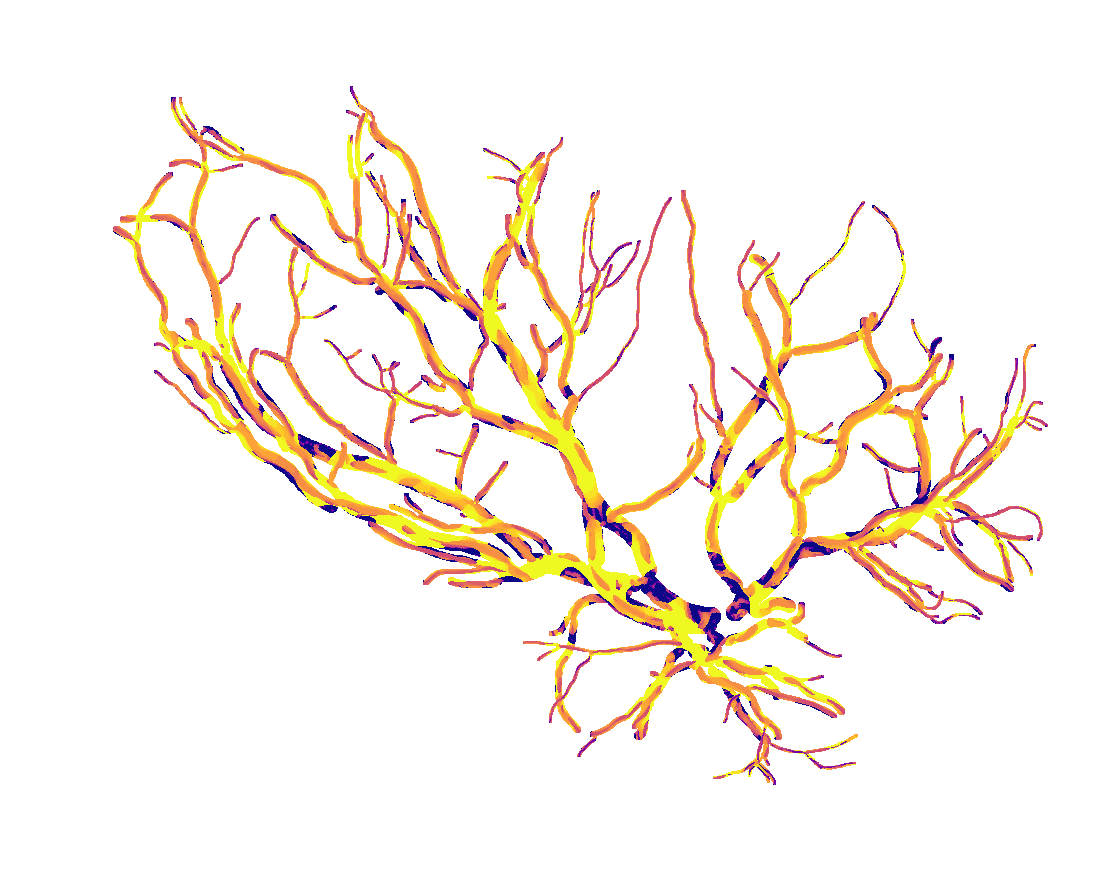
\includegraphics[width=0.85\textwidth]{frangi_argmax-trace}
  }
  \caption{Scale of maximum Frangi score for true positives and false negatives}
\end{figure}

\begin{figure}[p]\centering
  \subfloat{
    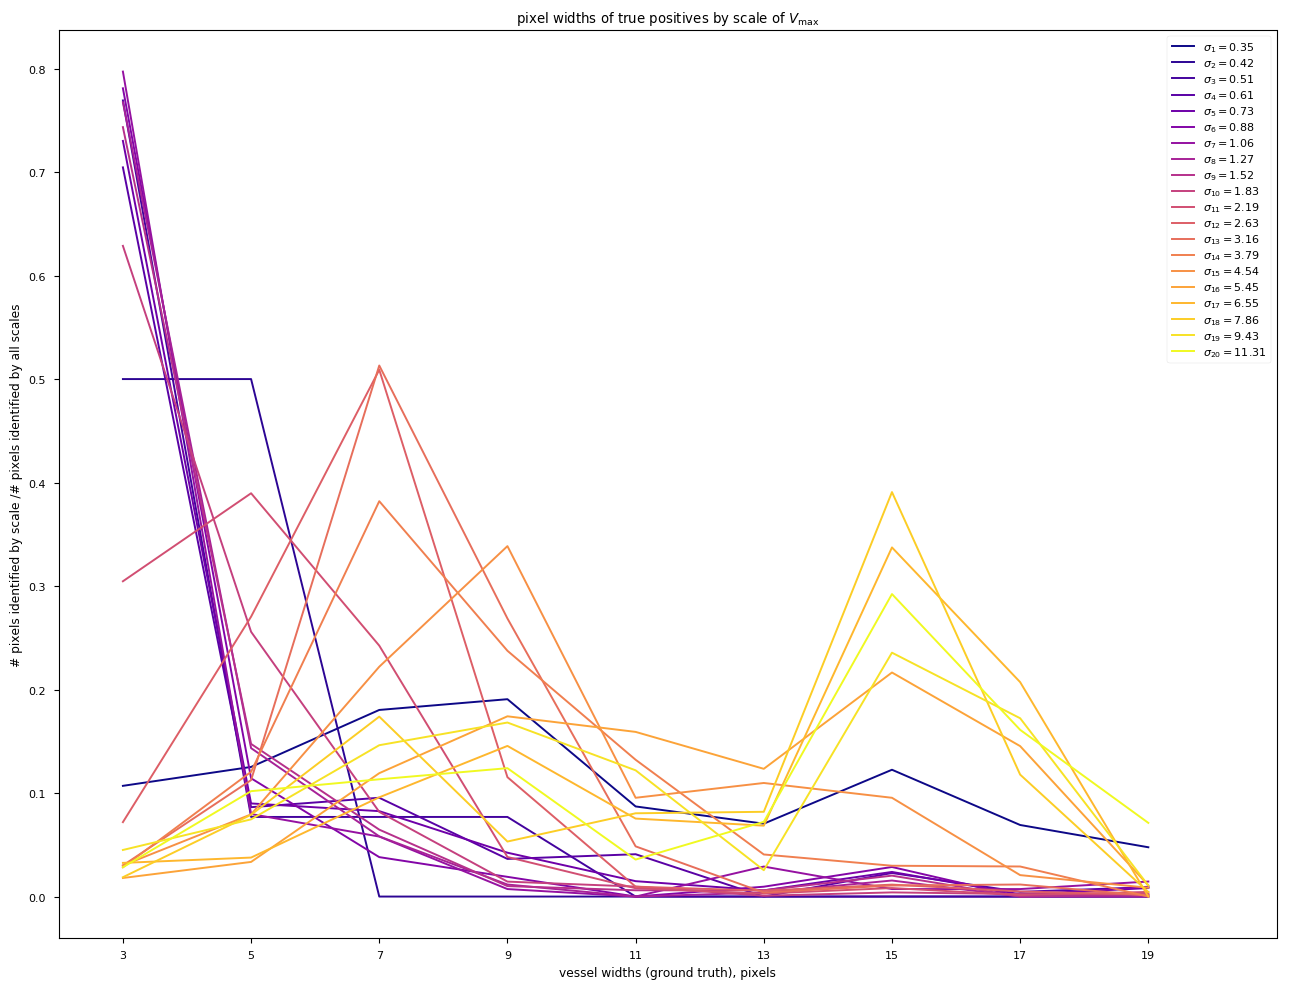
\includegraphics[width=0.85\textwidth]{Vmax_to_scale_normalized_with_approx}
  }\\[-0.5cm]
  \subfloat{
    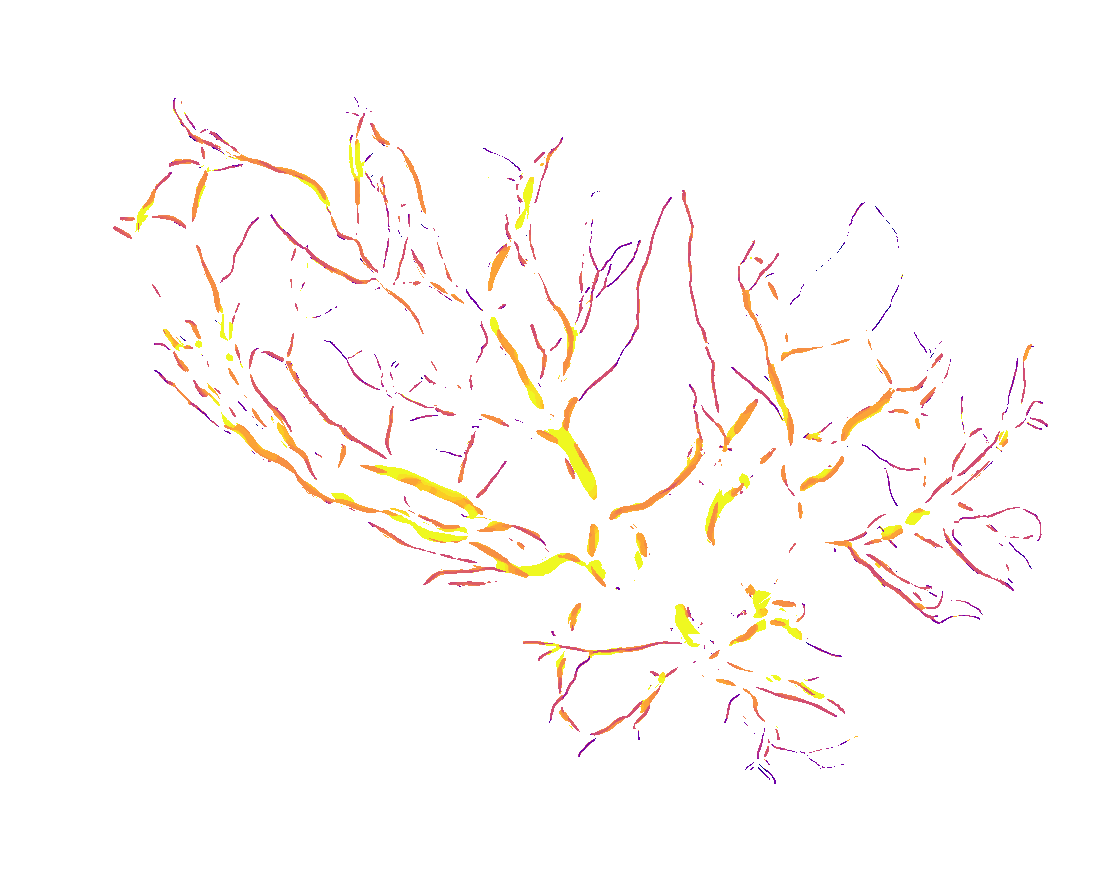
\includegraphics[width=0.85\textwidth]{frangi_argmax-trace-approx}
  }
  \caption{Scale of maximum Frangi score for true positives only (percentile filtering)}
\end{figure}
